\chapter{Design}
Angelina Scheler \& Christian Pfeiffer

\section{Einleitung}
Aufgabe des Design Teams war das Design der Stundenplanapp zu überarbeiten und zu verbessern, unter Berücksichtigung der Apple Human Interface Design Guideline. Dabei wurden für die V4 folgende Ziele gesetzt:

\begin{itemize}
\item Verbesserung der Stundenplanansicht
\item Design eines Onboarding Assistenten
\item Verbesserung und Vereinfachung der Einstellungen
\item Design eines Widgets
\item Entwicklung eines digitalen Prototypen
\end{itemize}


\section{Stundenplan}
Die Ansicht des Stundenplans ist das primäre Feature unserer Stundenplanapp. Deshalb ist es besonders wichtig, dieses stetig zu verbessern und zu erweitern.
Deshalb haben wir, um das Layout übersichtlicher zu gestalten, verschiedene Designkonzepte entworfen.

\subsection{Vorschlag zur Verbesserung der Usability der Stundenplanansicht}
Zu Beginn des Semesters wurde ein Konzept entwickelt, innerhalb dessen die Stundenplanfunktion durch eine Wochenansicht erweitert werden sollte. 

\begin{figure}[H]
	\centering
  \frame{ 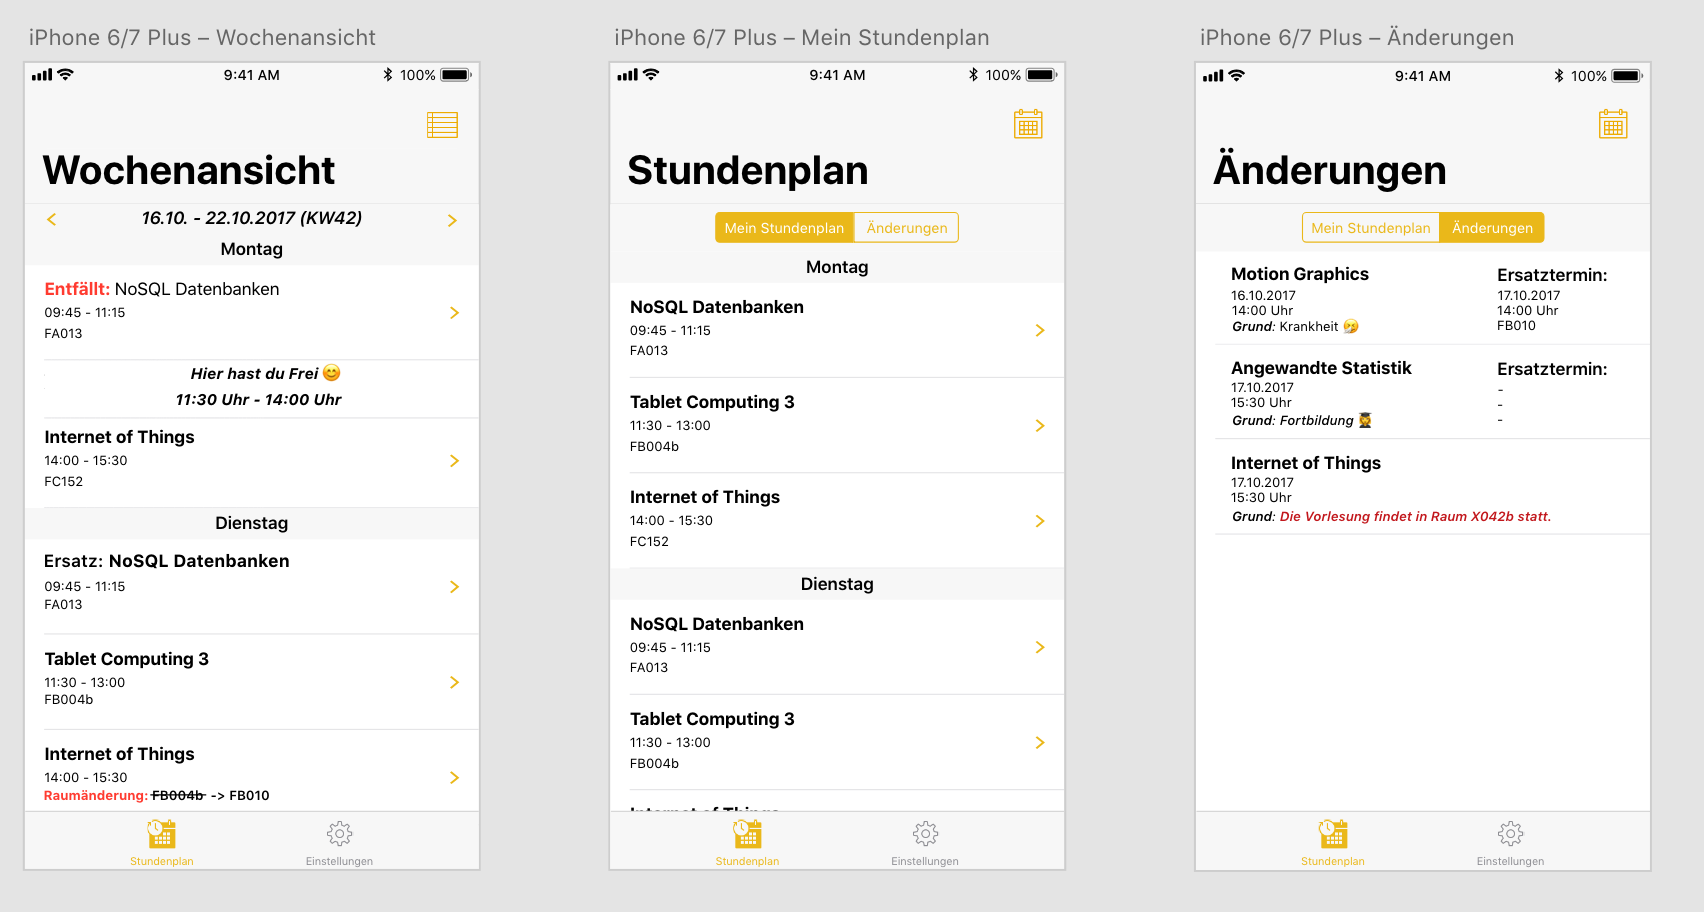
\includegraphics[scale=0.5]{design_stundenplan}}
	\caption{Neues Stundenplanbedienkonzept}
	\label{fig1}
\end{figure}

Mit dem rechten oberen Navigationitem kann zwischen einer Wochenansicht und der klassischen Stundenplanansicht gewechselt werden. In der klassischen Stundenplanansicht kann der Benutzer durch ein ein Segmented Control Element unterhalb der Navigationbar zwischen 'Mein Stundenplan'' und den Stundenplanänderungen wechseln. In der Wochenansicht werden ''Mein Stundenplan'' und die Stundenplanänderungen in einer Ansicht für die aktuelle Woche kombiniert dargestellt. 

\subsection{Entwicklung eines neuen Farbdesigns mit neuem Layout der Zellen}
In der vorherigen Version der Stundenplanapp hatte jede Funktion eine eigene, dem Hochschulfakultäten entsprechende, Farbe. Da das Wechseln der Farbe, bei Auswahl einer neuen Funktion inkonsistent ist, hat das Designteam ein Konzept entwickelt, durch welches der Appnutzer in den Einstellungen seine Fakultät wählen kann und die App damit mit der gewählten Fakultätsfarbe anpassen kann. 
Die folgenden Abbildungen zeigen die Stundenplanansicht in den jeweiligen Fakultätsfarben. Das Layout der Stundenplanzellen wurde darüber hinaus auch verbessert. 

\begin{figure}[H]
	\centering
  \frame{ 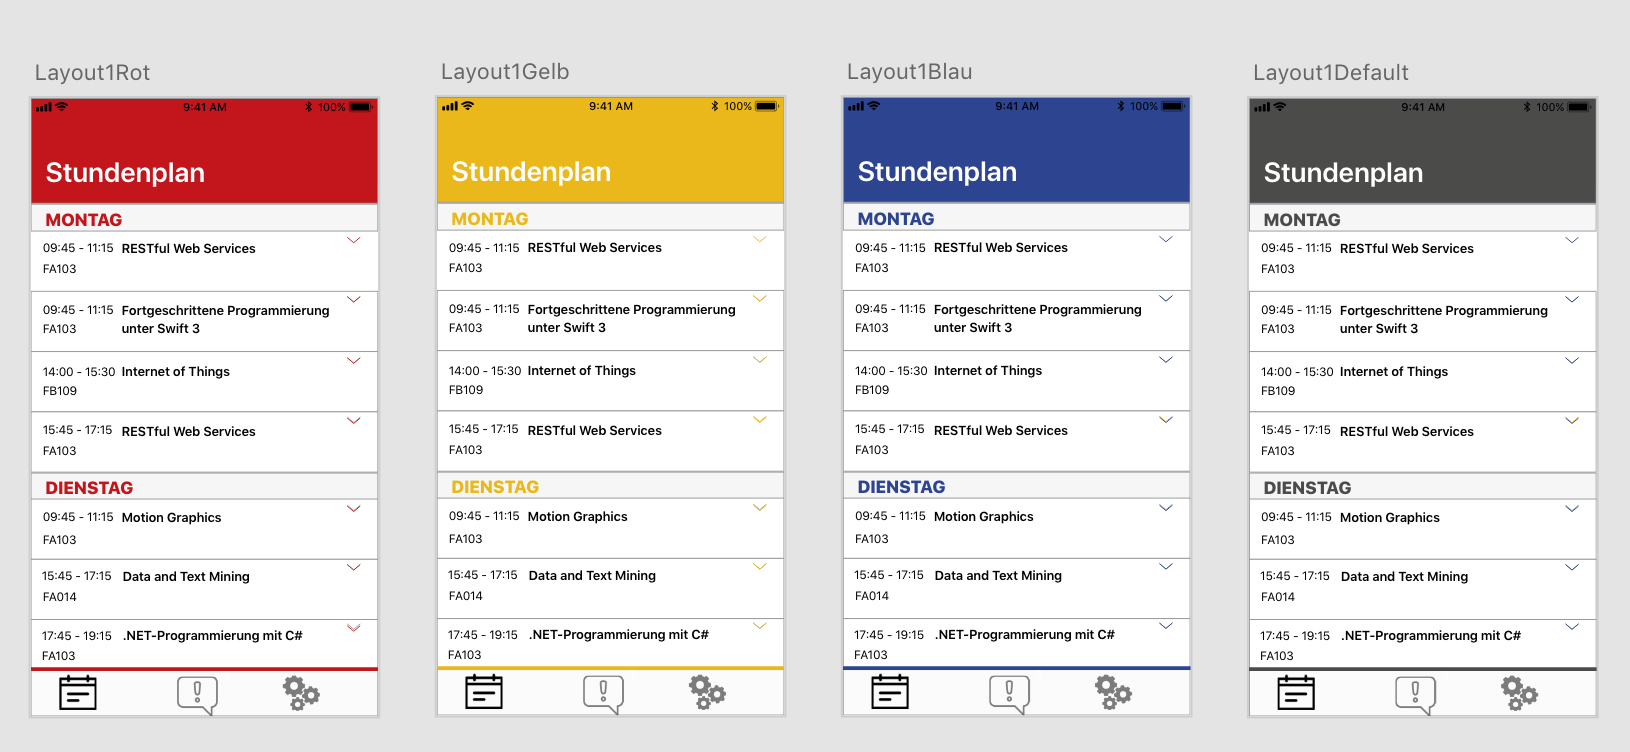
\includegraphics[scale=0.5]{Design1}}
	\caption{Design Konzept 1, Stundenplan Ansicht}
	\label{fig1}
\end{figure}

\begin{figure}[H]
	\centering
  \frame{ 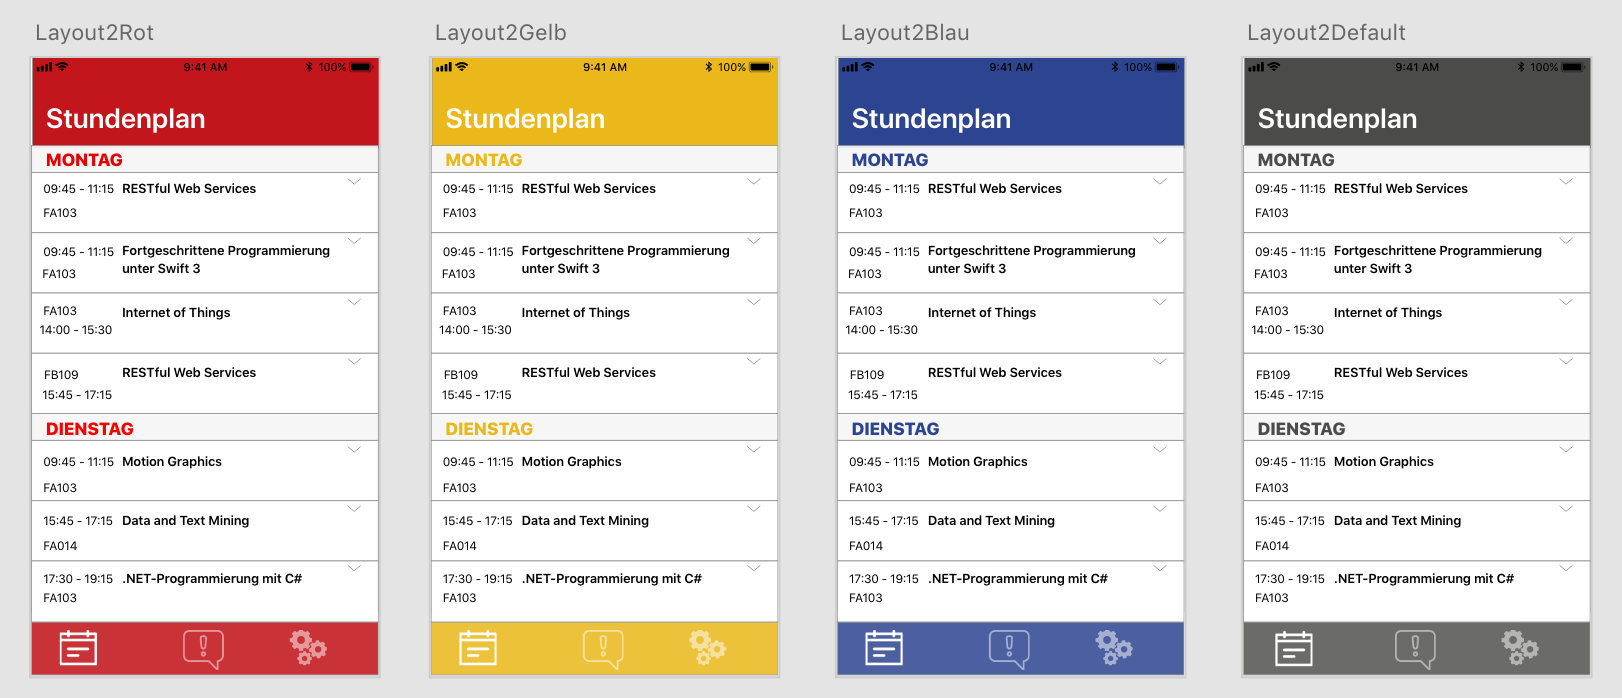
\includegraphics[scale=0.5]{Design2}}
	\caption{Design  Konzept 2, Stundenplan Ansicht}
	\label{fig1}
\end{figure}

\begin{figure}[H]
	\centering
  \frame{ 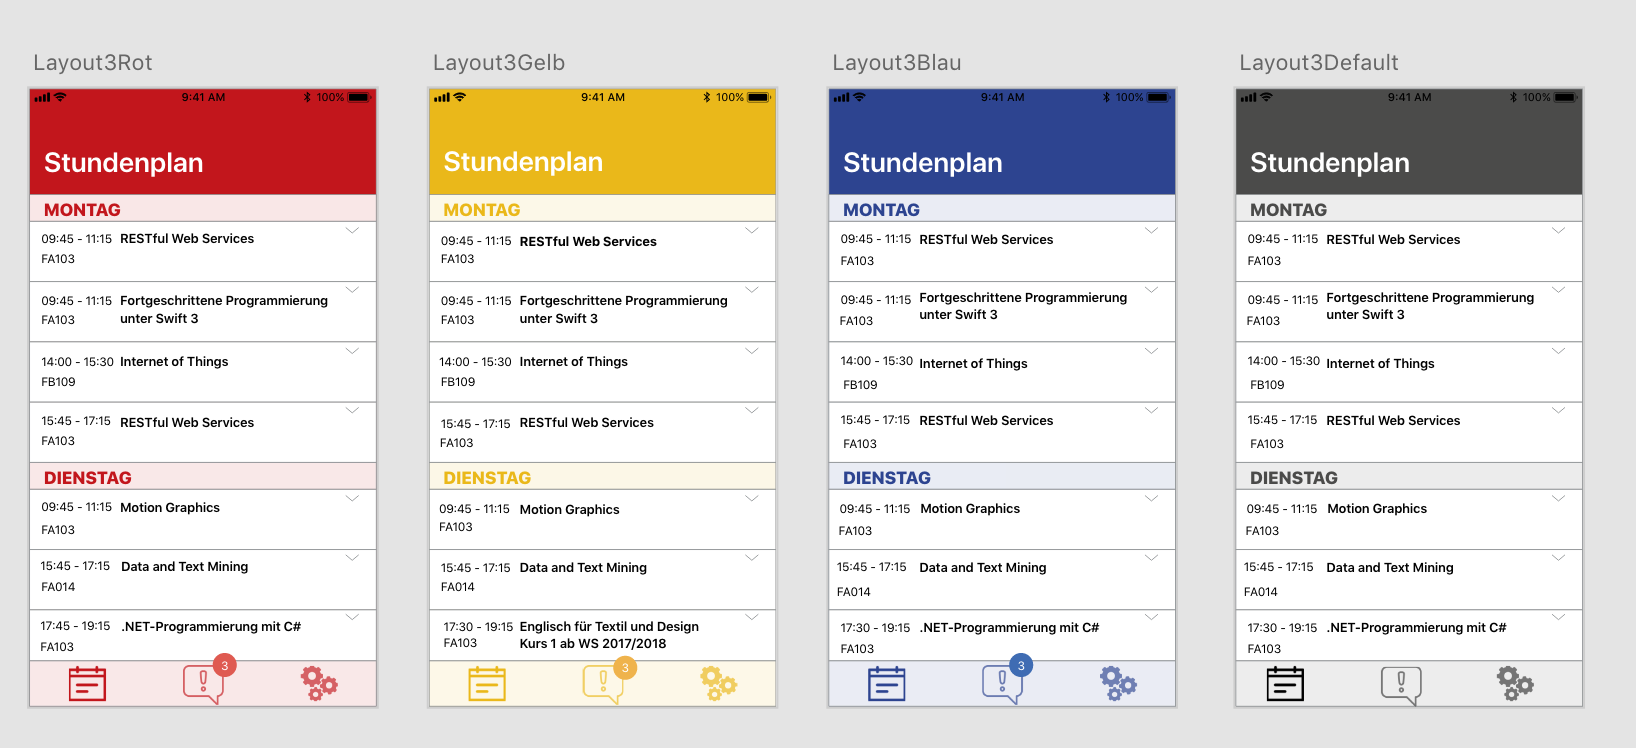
\includegraphics[scale=0.5]{Design3}}
	\caption{Design Konzept 3,  Stundenplan Ansicht}
	\label{fig1}
\end{figure}

\begin{figure}[H]
	\centering
  \frame{ 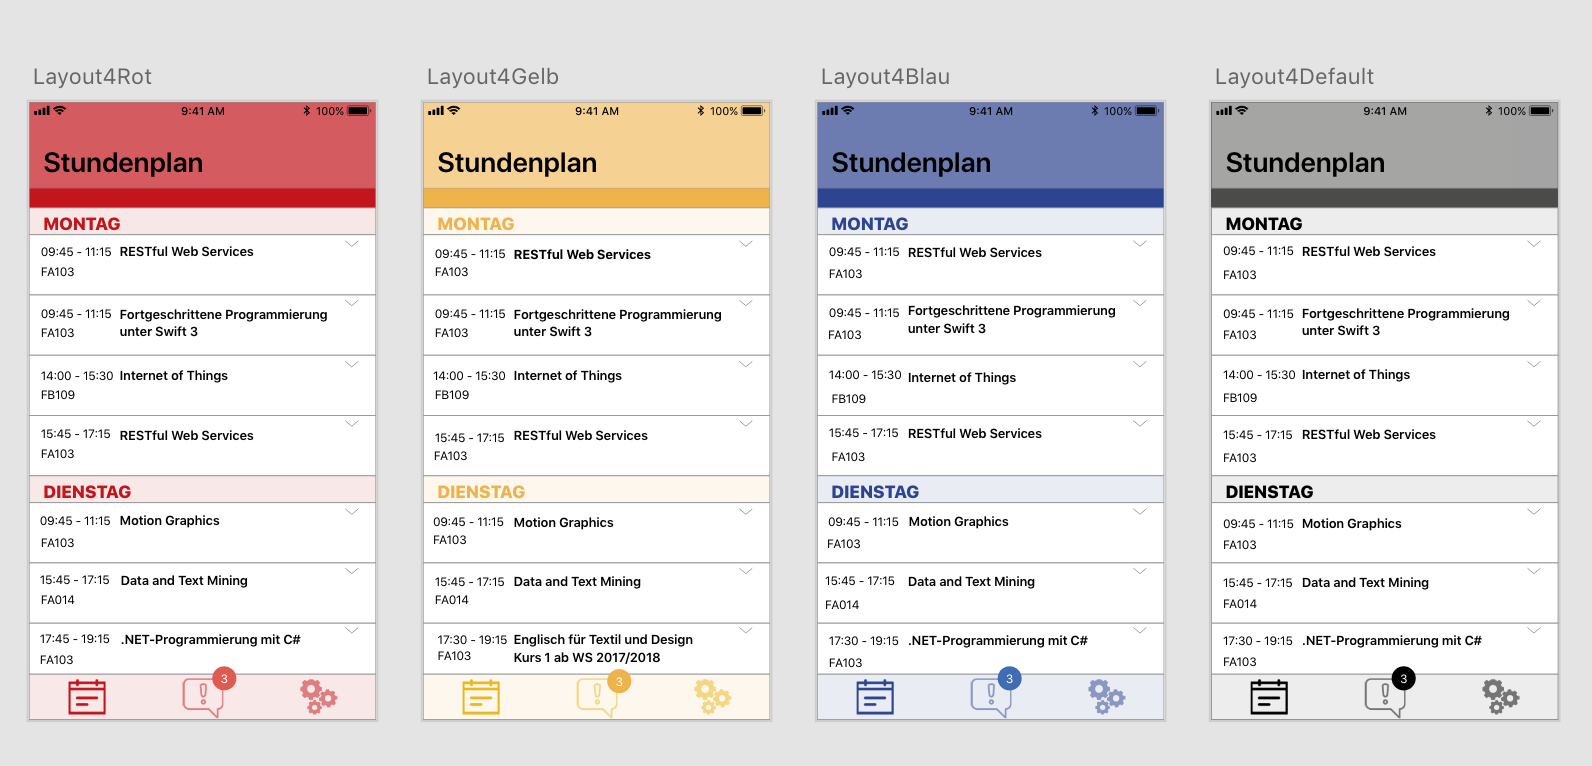
\includegraphics[scale=0.5]{Design4}}
	\caption{Design Konzept 4,  Stundenplan Ansicht}
	\label{fig1}
\end{figure}

\subsection{Finales Design}
Das Finale Design ist ein Kompromiss aus Altem und Neuem Layout, die Fakultätsfarben wurden eingeführt, Informationen übersichtlicher positioniert und farblich angepasst.

\begin{figure}[H]
	\centering
  \frame{ 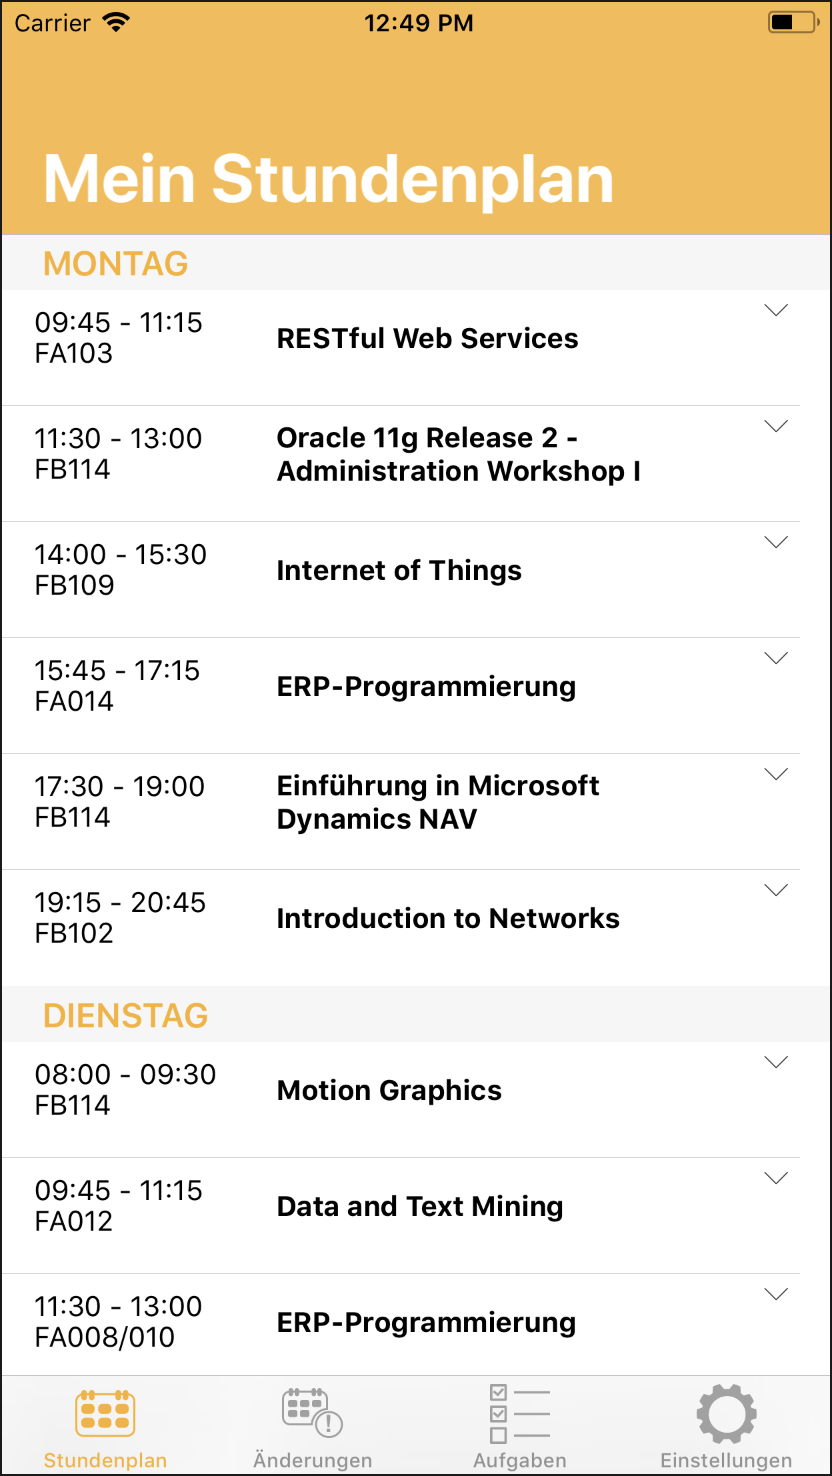
\includegraphics[scale=0.3]{FinalesDesignStundenplan}}
	\caption{Finales Design, Stundenplan Ansicht}
	\label{fig1}
\end{figure}

\section{Onboarding}

Um neuen Appnutzern eine geführte Einführung in die Funktionalität und Einstellungsmöglichkeiten zu bieten, ist die Implementation einer Onboardingfunktion sinnvoll. Deshalb wurden Mockups einer solchen Funktion entwickelt, die einen solchen Onboardingprozess darstellen.

\begin{figure}[H]
	\centering
  \frame{ 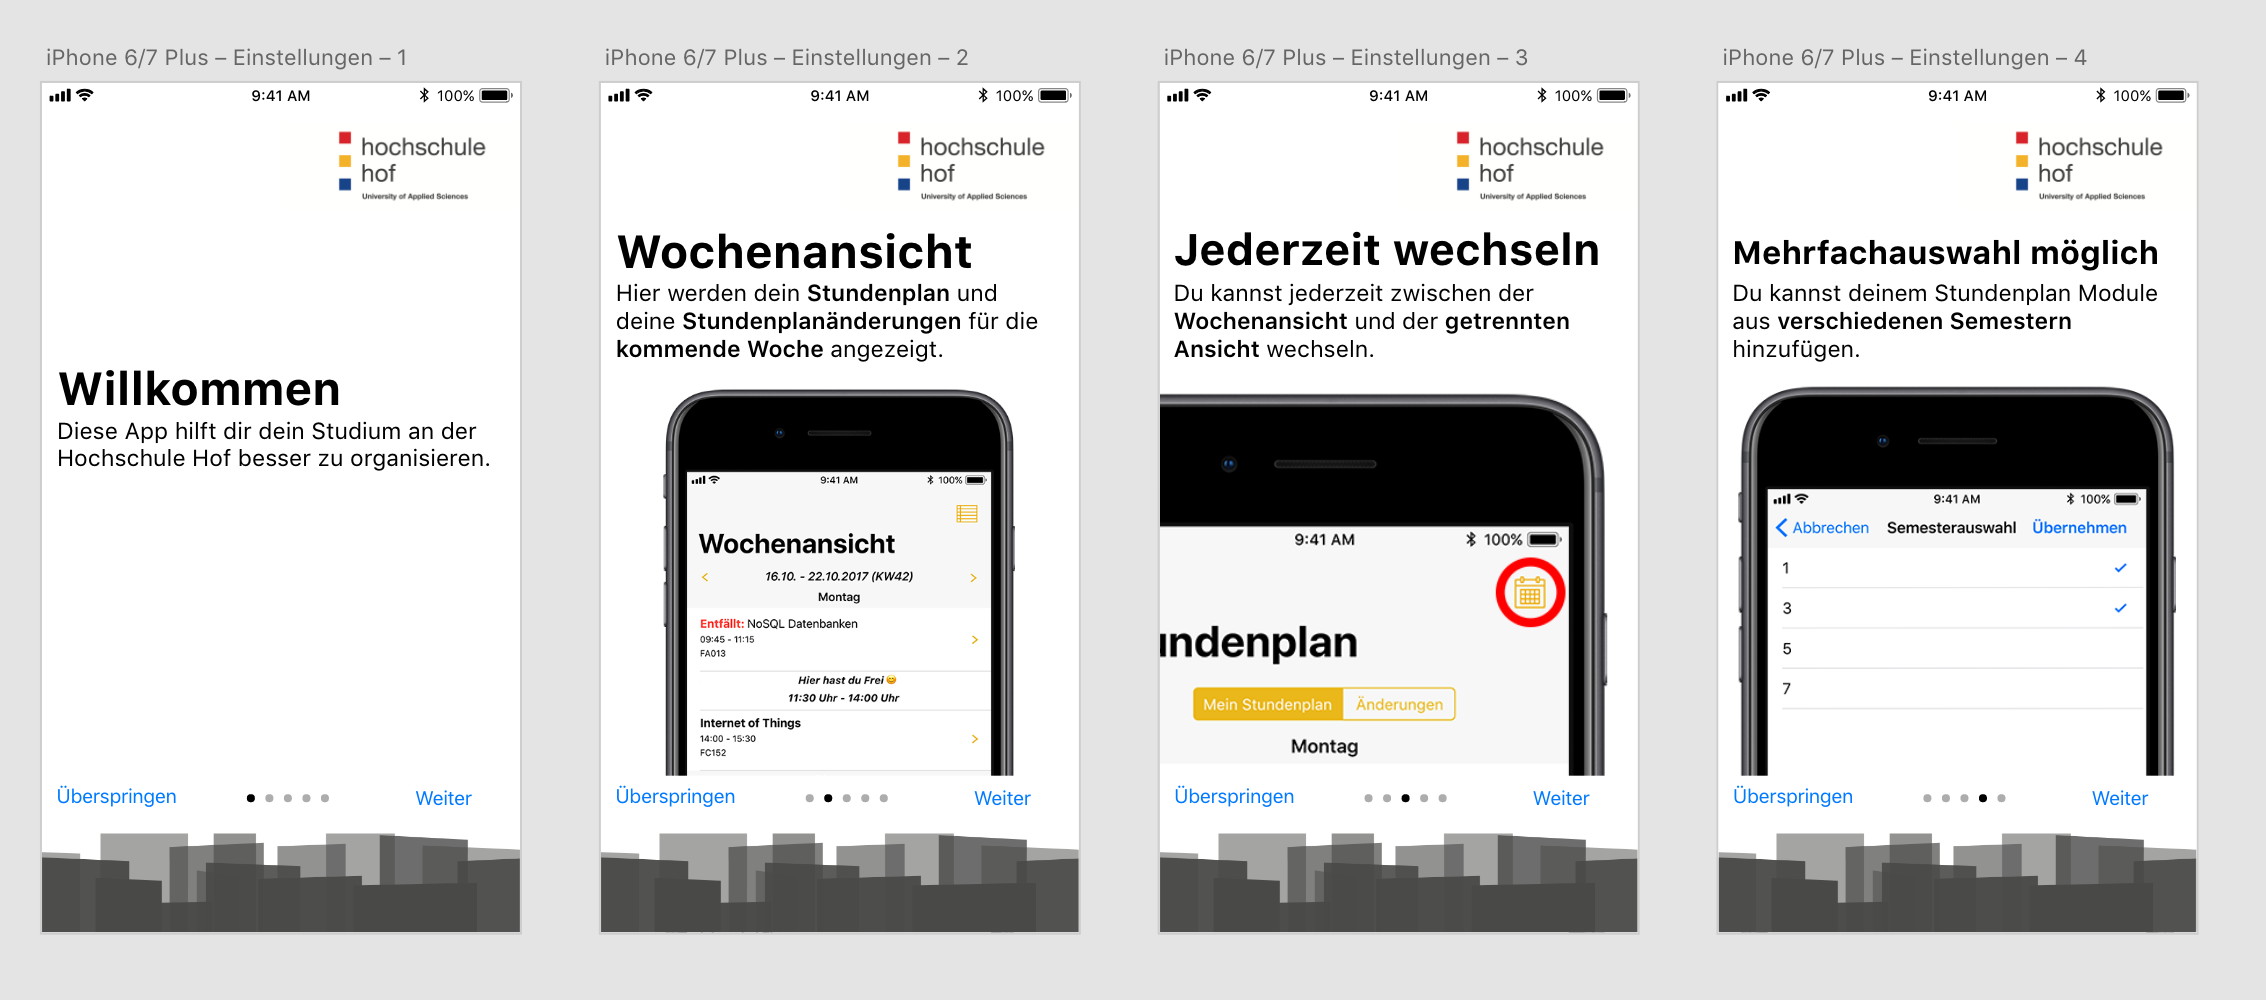
\includegraphics[scale=0.4]{design_onboarding1}}
	\caption{Onboardingkonzeptmockup}
	\label{fig1}
\end{figure}

\begin{figure}[H]
	\centering
  \frame{ 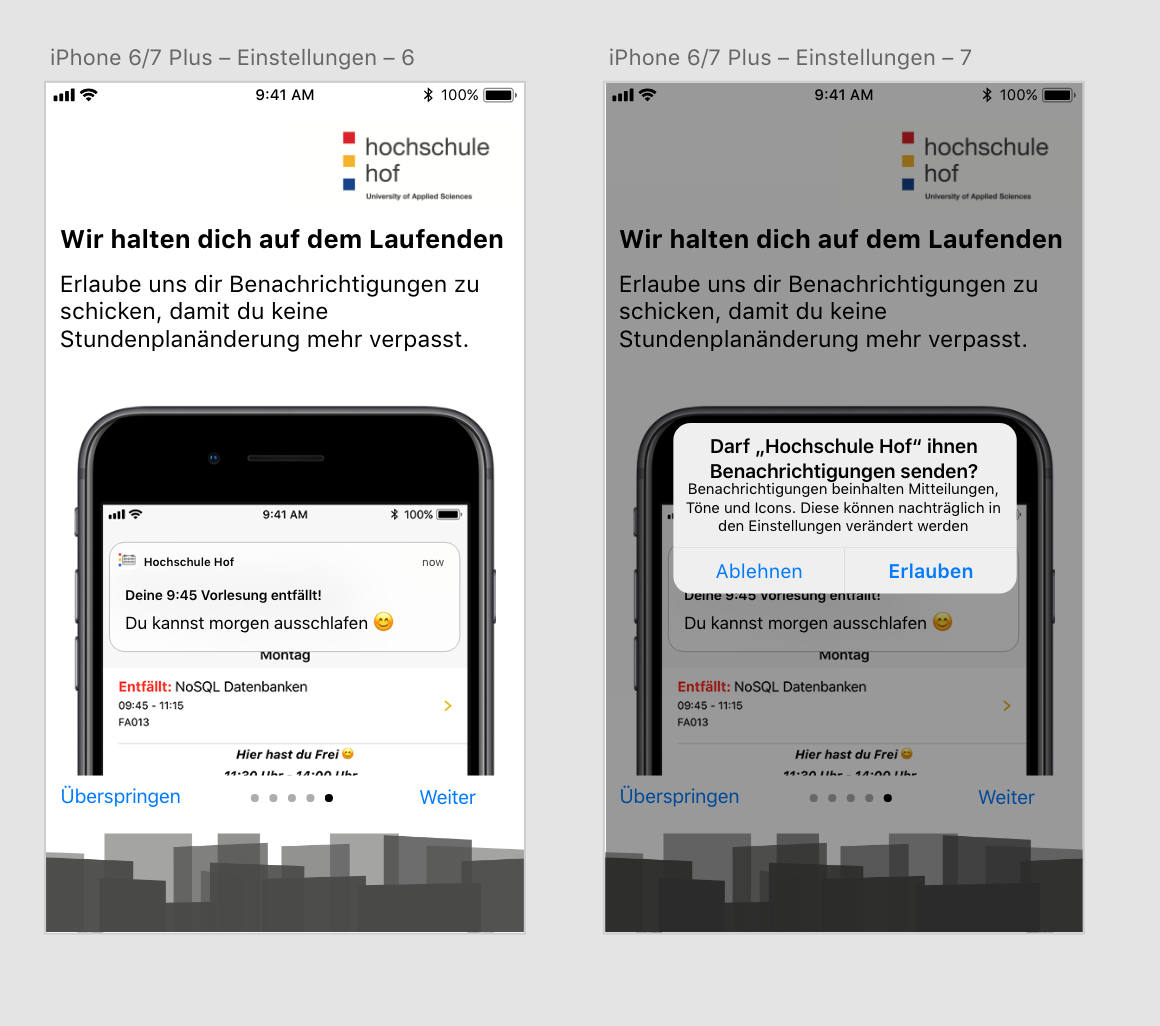
\includegraphics[scale=0.5]{design_onboarding2}}
	\caption{Onboardingkonzeptmockup}
	\label{fig1}
\end{figure}

\subsection{finales Design}
\begin{figure}[H]
	\centering
  \frame{ 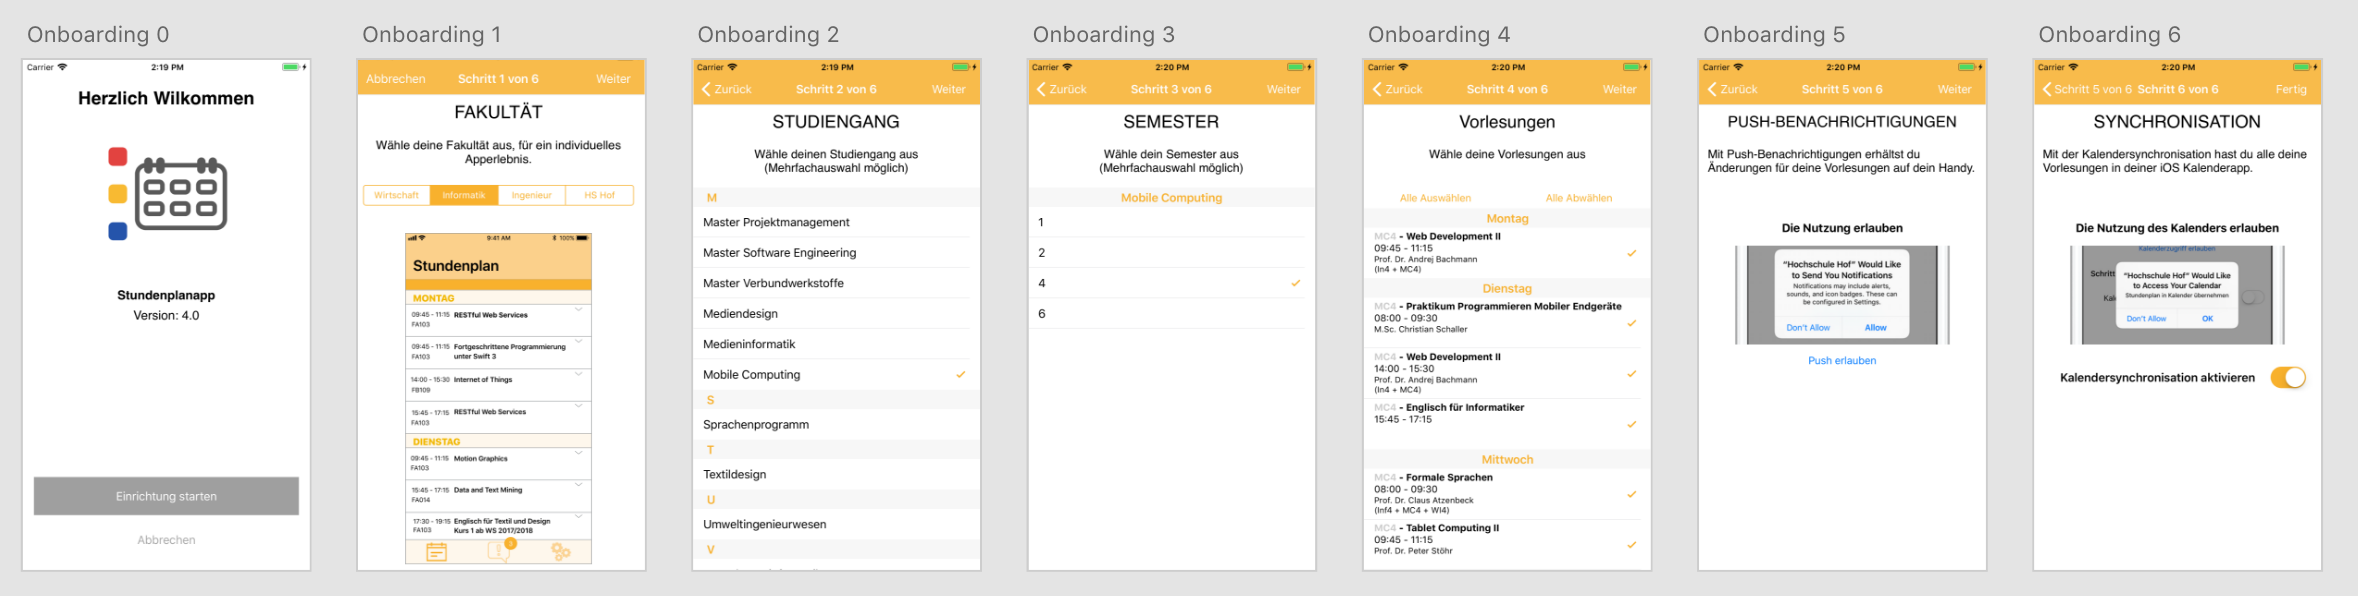
\includegraphics[scale=0.4]{design_onboarding3}}
	\caption{finale Implementierung des Onboarding}
	\label{fig1}
\end{figure}

Beim ersten Start der App, wird der Nutzer von der App begrüßt und kann sich entscheiden, ober er das Onboarding durchführen möchte, oder es lieber überspringen möchte. Falls er sich entschließt, dass Onboarding durchzuführen, kann er auf dem nächsten Bildschirm eine seiner Lieblingsfakultät entsprechenden App Farbe entscheiden. Im darauffolgenden Schritt, müssen der/die Studiengang/Studiengägne ausgewählt werden und anschließend das/die Semester.  Im 4. Schritt können die Vorlesungen gewählt werden. In den letzten zwei Schritten werden dem Benutzer die Vorteile von Push Notifications und der Kalendersyncronisation erklärt. Hier kann er jeweils die Entscheidung treffen diese Funktionen zu aktivieren und der App dafür die benötigten iOS Berechtigungen erteilen. Nach erfolgtem Onboarding schließt sich der Onboarding Assistent und der Benutzer befindet sich in den Einstellungen.



\section{Einstellungen}
Das Vornehmen von Einstellungen ist ein wichtiger Bestandteil unserer Stundenplanapp, deshalb ist es wichtig in diesem Bereich ein Konzept zu entwickeln, welches dem Appnutzer eine gute Übersicht, sowie die für ihn wichtigen Schritte zu den Einstellungen so effizient wie möglich präsentiert.

\subsection{Vereinfachung der Stundenplanauswahl}
In der vorherigen Versionen der Stundenplanapp, war die Auswahl eines persönlichen Stundenplans zu kompliziert und zu langwierig. Deswegen wurde ein Konzept entwickelt, mithilfe dessen ein personalisierter Stundenplan in einem Schritt weniger und mit weniger Einstellungselemente  ausgewählt werden kann.

\begin{figure}[H]
	\centering
  \frame{ 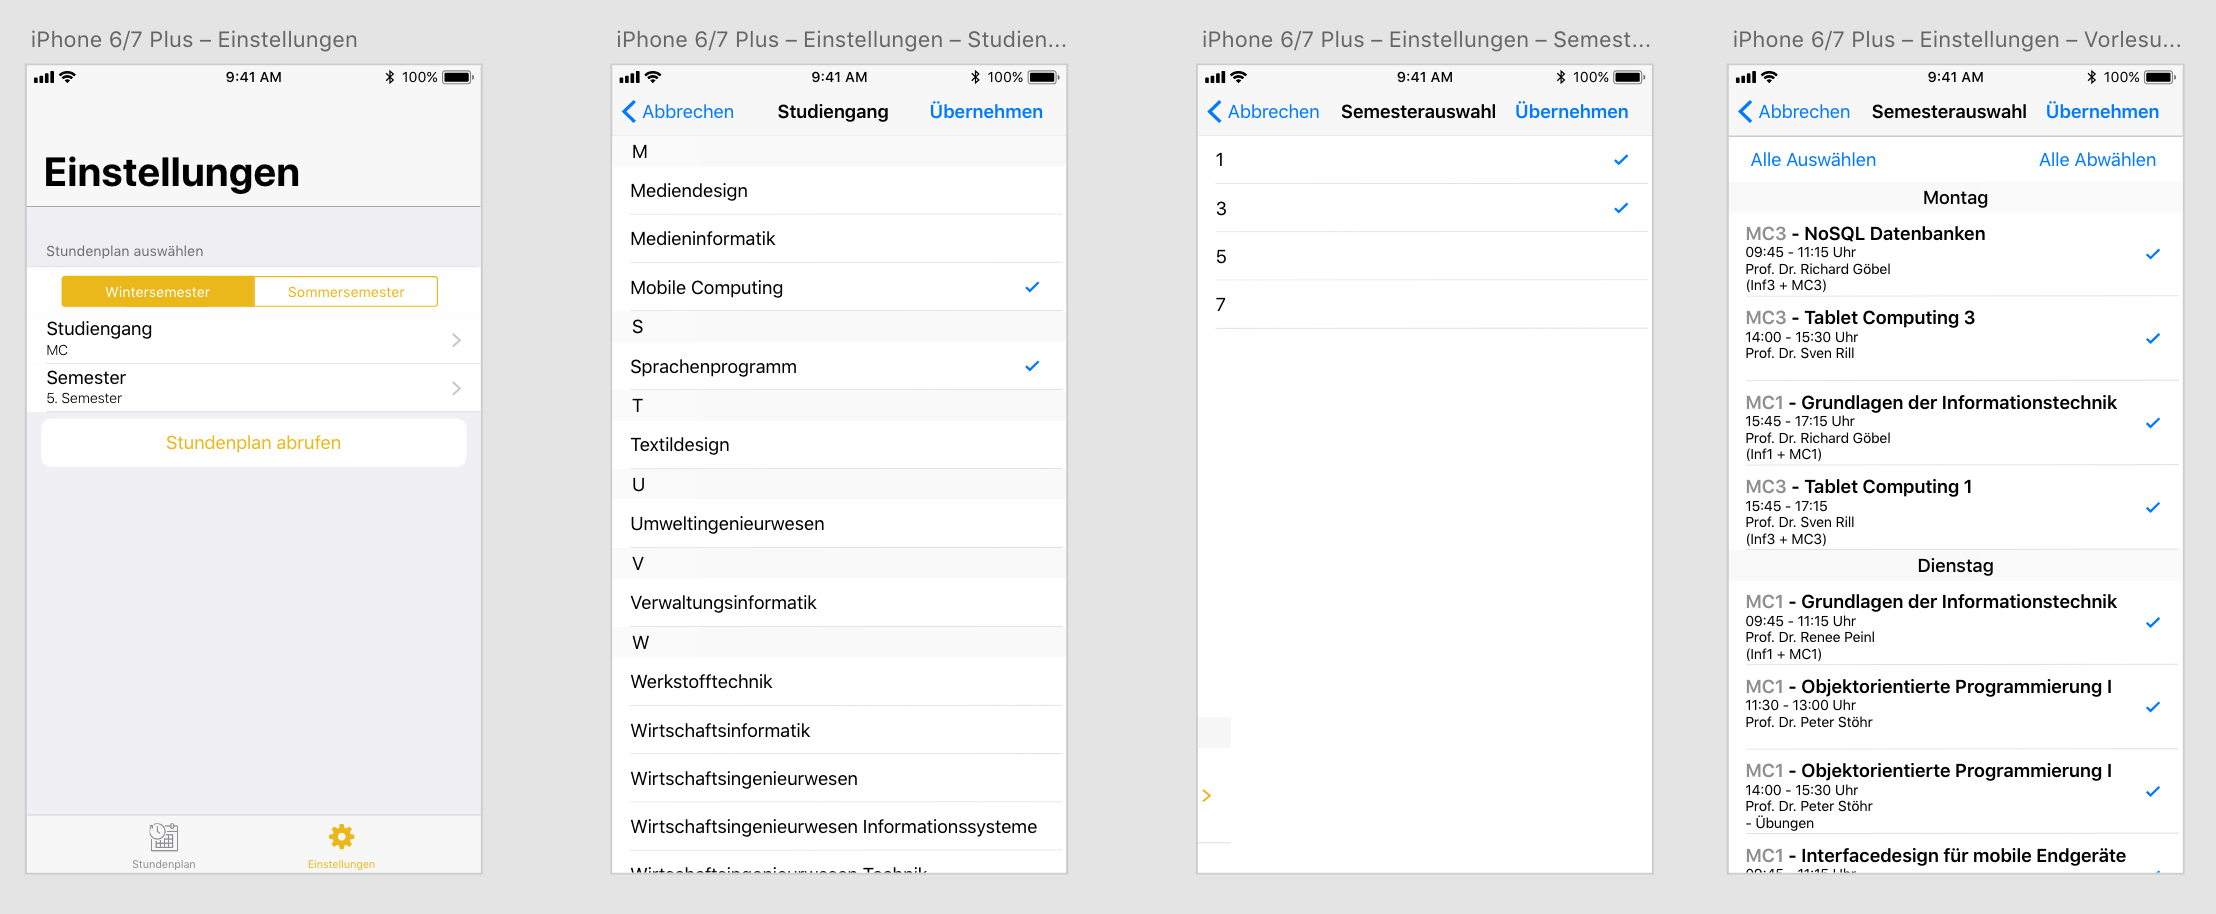
\includegraphics[scale=0.4]{design_settings}}
	\caption{Optimierung der Schritte zur Stundenplanauswahl auf die nötigsten Schritte}
	\label{fig1}
\end{figure}

Im Gegensatz zur vorherigen Version fällt mit diesem Konzept der Schritt des Bestätigen des Stundenplanes auf dem Einstellungsbildschirm weg. Stattdessen werden die ausgewählten Vorlesungen in der Push Over View der Vorlesungsauswahl bestätigt. Die Vorlesungsauswahl ist auch keine Table View Zelle mehr, sondern ein Button. Der Button zum Bestätigen der Ausgewählten Vorlesungen entfällt ebenso.

\subsection{Design Vorschlag}

\begin{figure}[H]
	\centering
  \frame{ 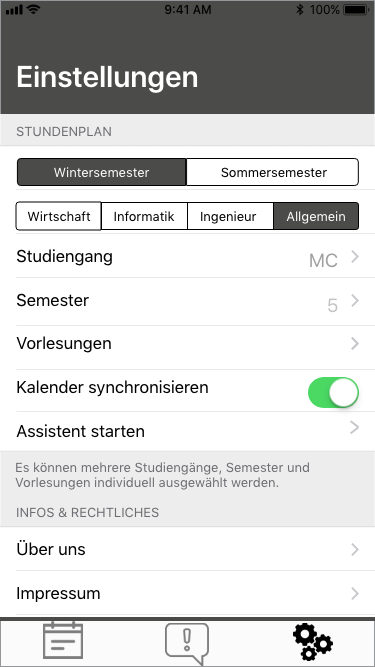
\includegraphics[scale=0.5]{Layout1Settings}}
	\caption{Design Konzept, Stundenplan Einstellungen}
	\label{fig1}
\end{figure}

\subsection{Design Umsetzung}
Es wurde ein Menüpunkt für die Fakultätsauswahl und starten des Einführungsassistenten eingefügt. Desweiteren wurden in den jeweiligen Einstellungsscreens wie, Studiengang, Semester und Vorlesungen anpassungen vorgenommen, wie die Alphabetisierung siehe Abbildung 2.8.. Außerdem wurden alle Inhalte je nach Fakultätsauswahl farblich angepasst.

\begin{figure}[H]
	\centering
  \frame{ 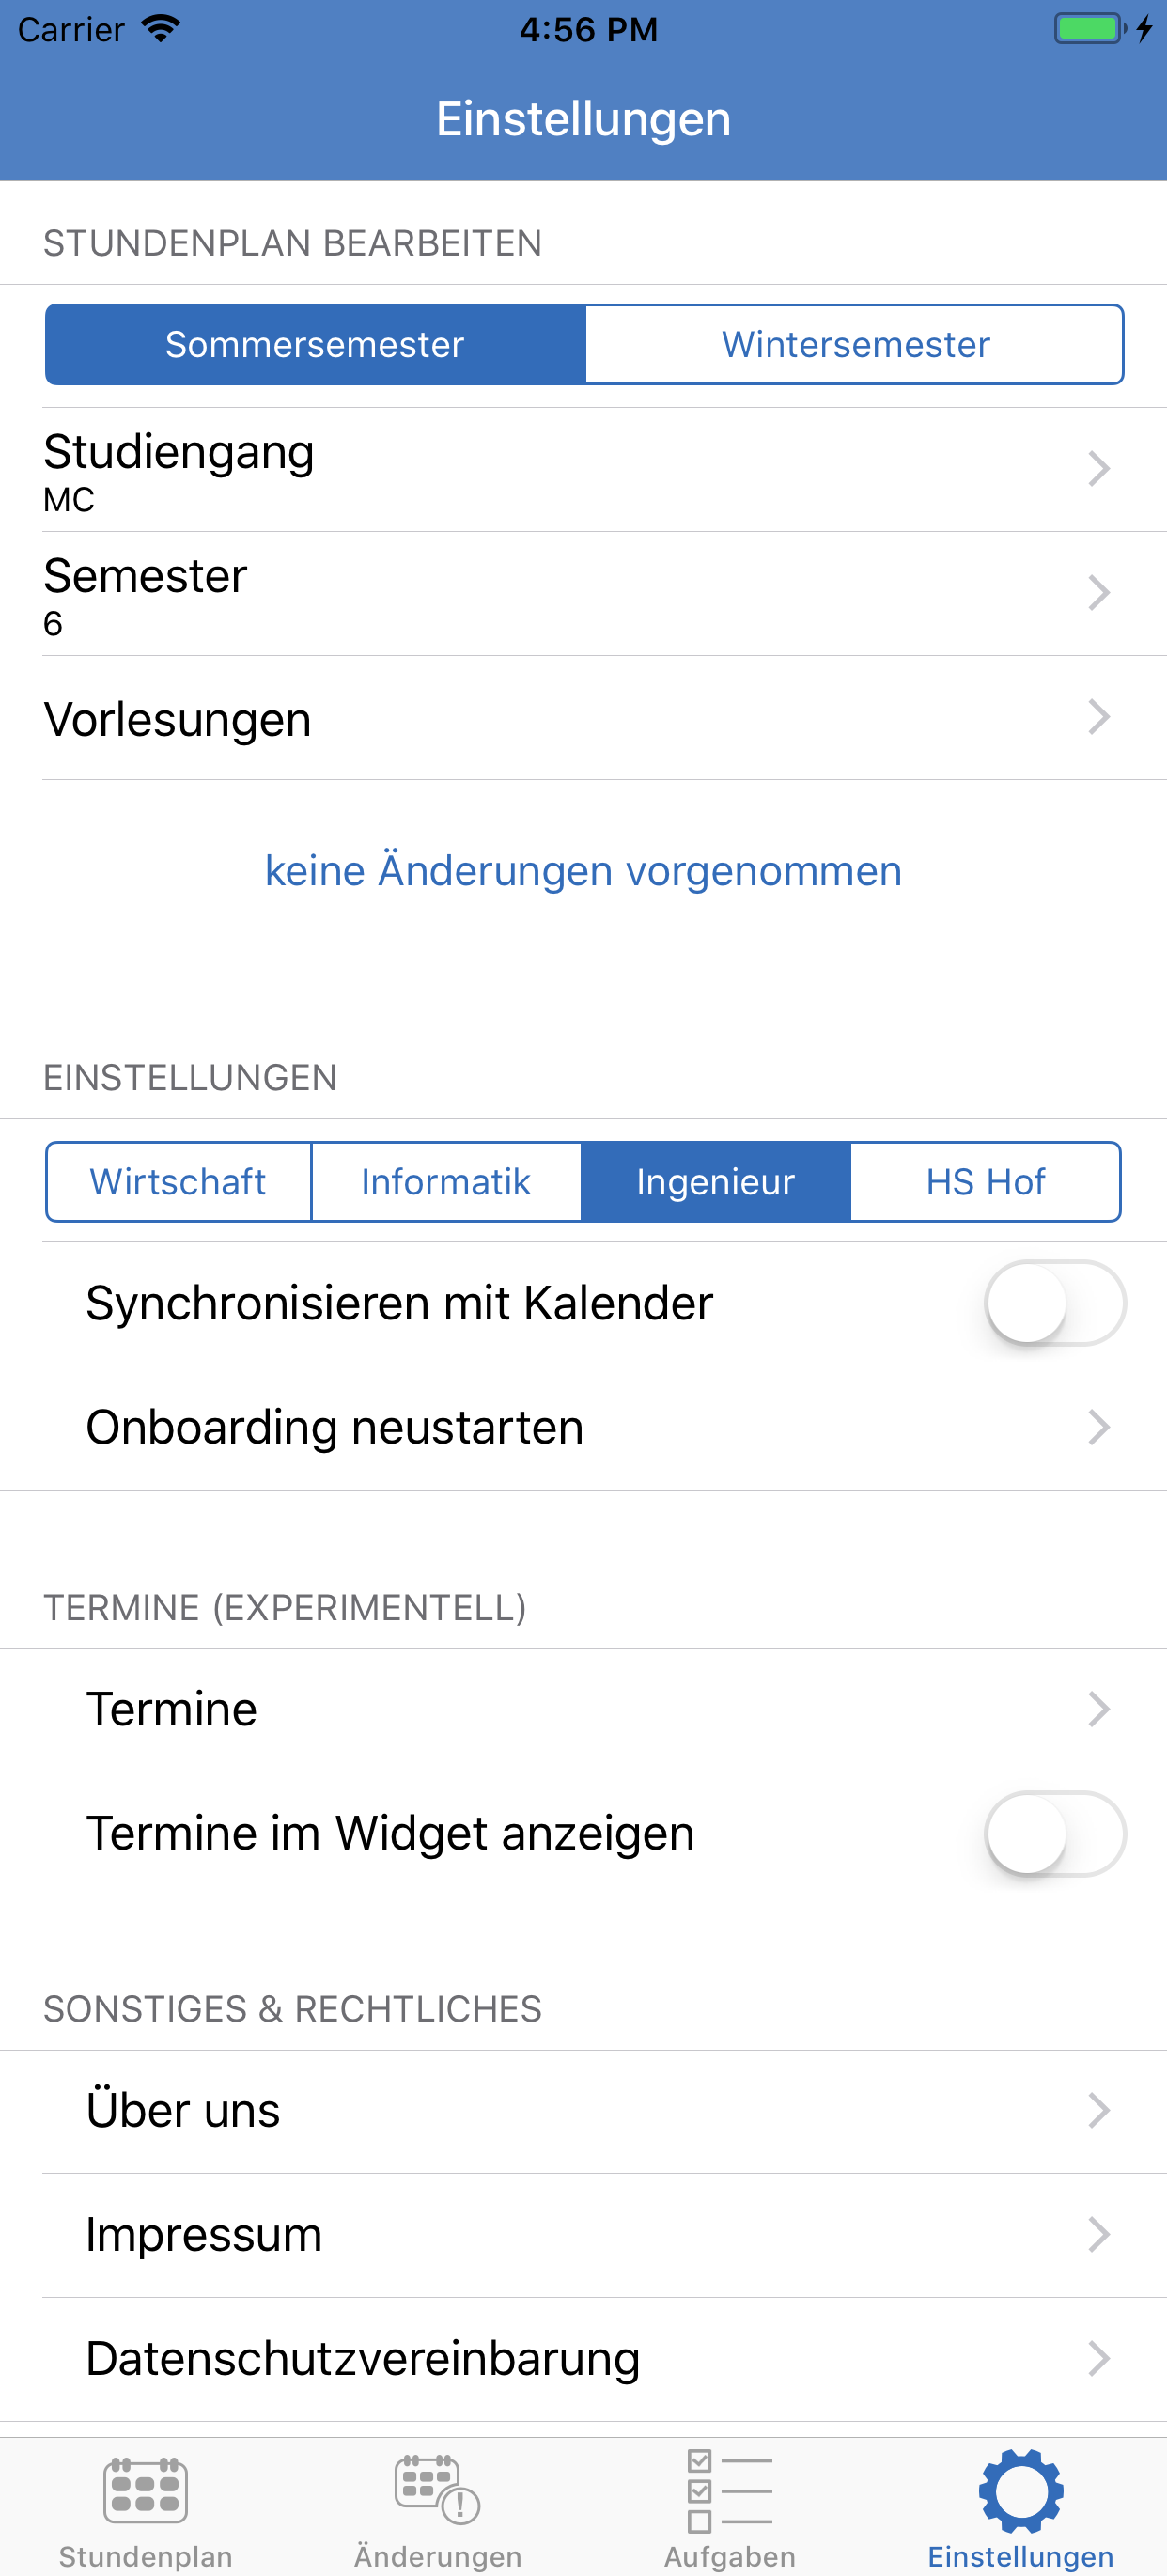
\includegraphics[scale=0.15]{FinalesDesignSettings}}
	\caption{Finales Design, Stundenplan Einstellungen}
	\label{fig1}
\end{figure}

In der finalen Version wurden, die Einstellungsmöglichkeiten neu angeordnet, sowie einige Einstellungen (Onboarding neustarten, Auswahl einer Fakultätsfarbe, Termine, Widget etc.) hinzugefügt.

\section{Widget}

\subsection{Design Widget}
\begin{figure}[H]
	\centering
  \frame{ 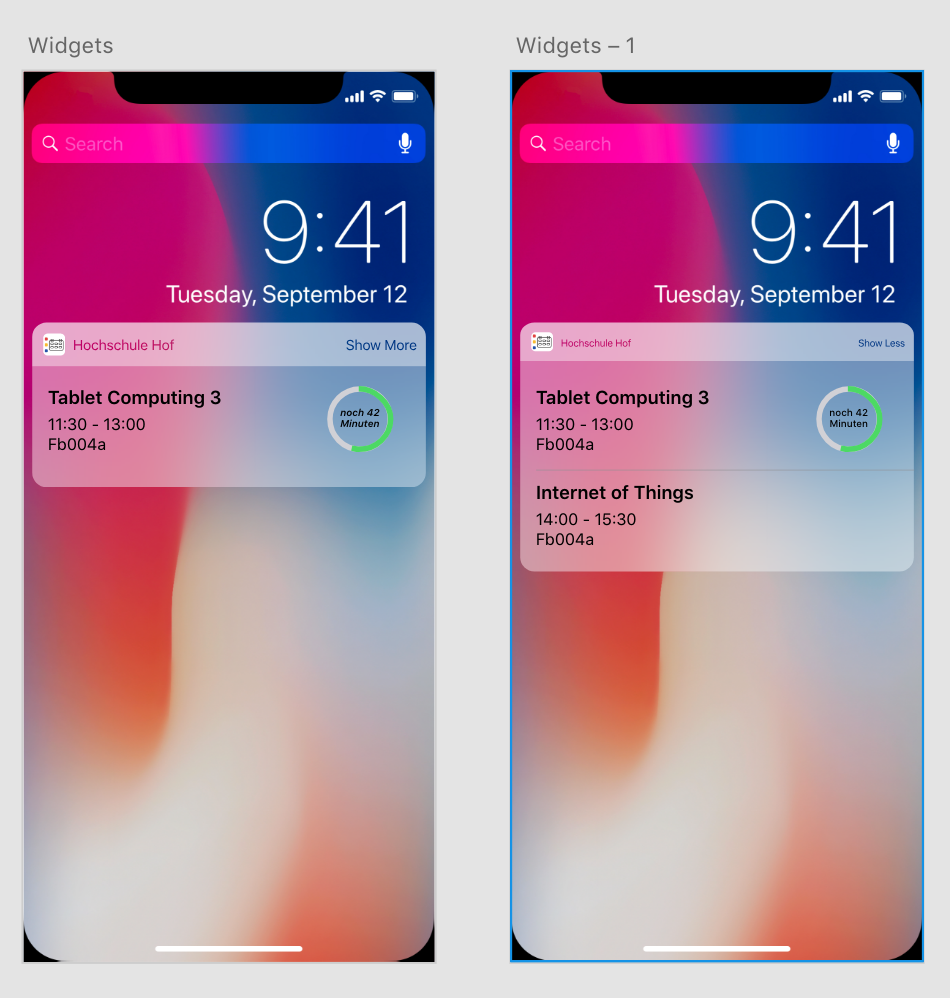
\includegraphics[scale=0.5]{design_widget}}
	\caption{Design  Widget 1}
	\label{fig1}
\end{figure}

\begin{figure}[H]
	\centering
  \frame{ 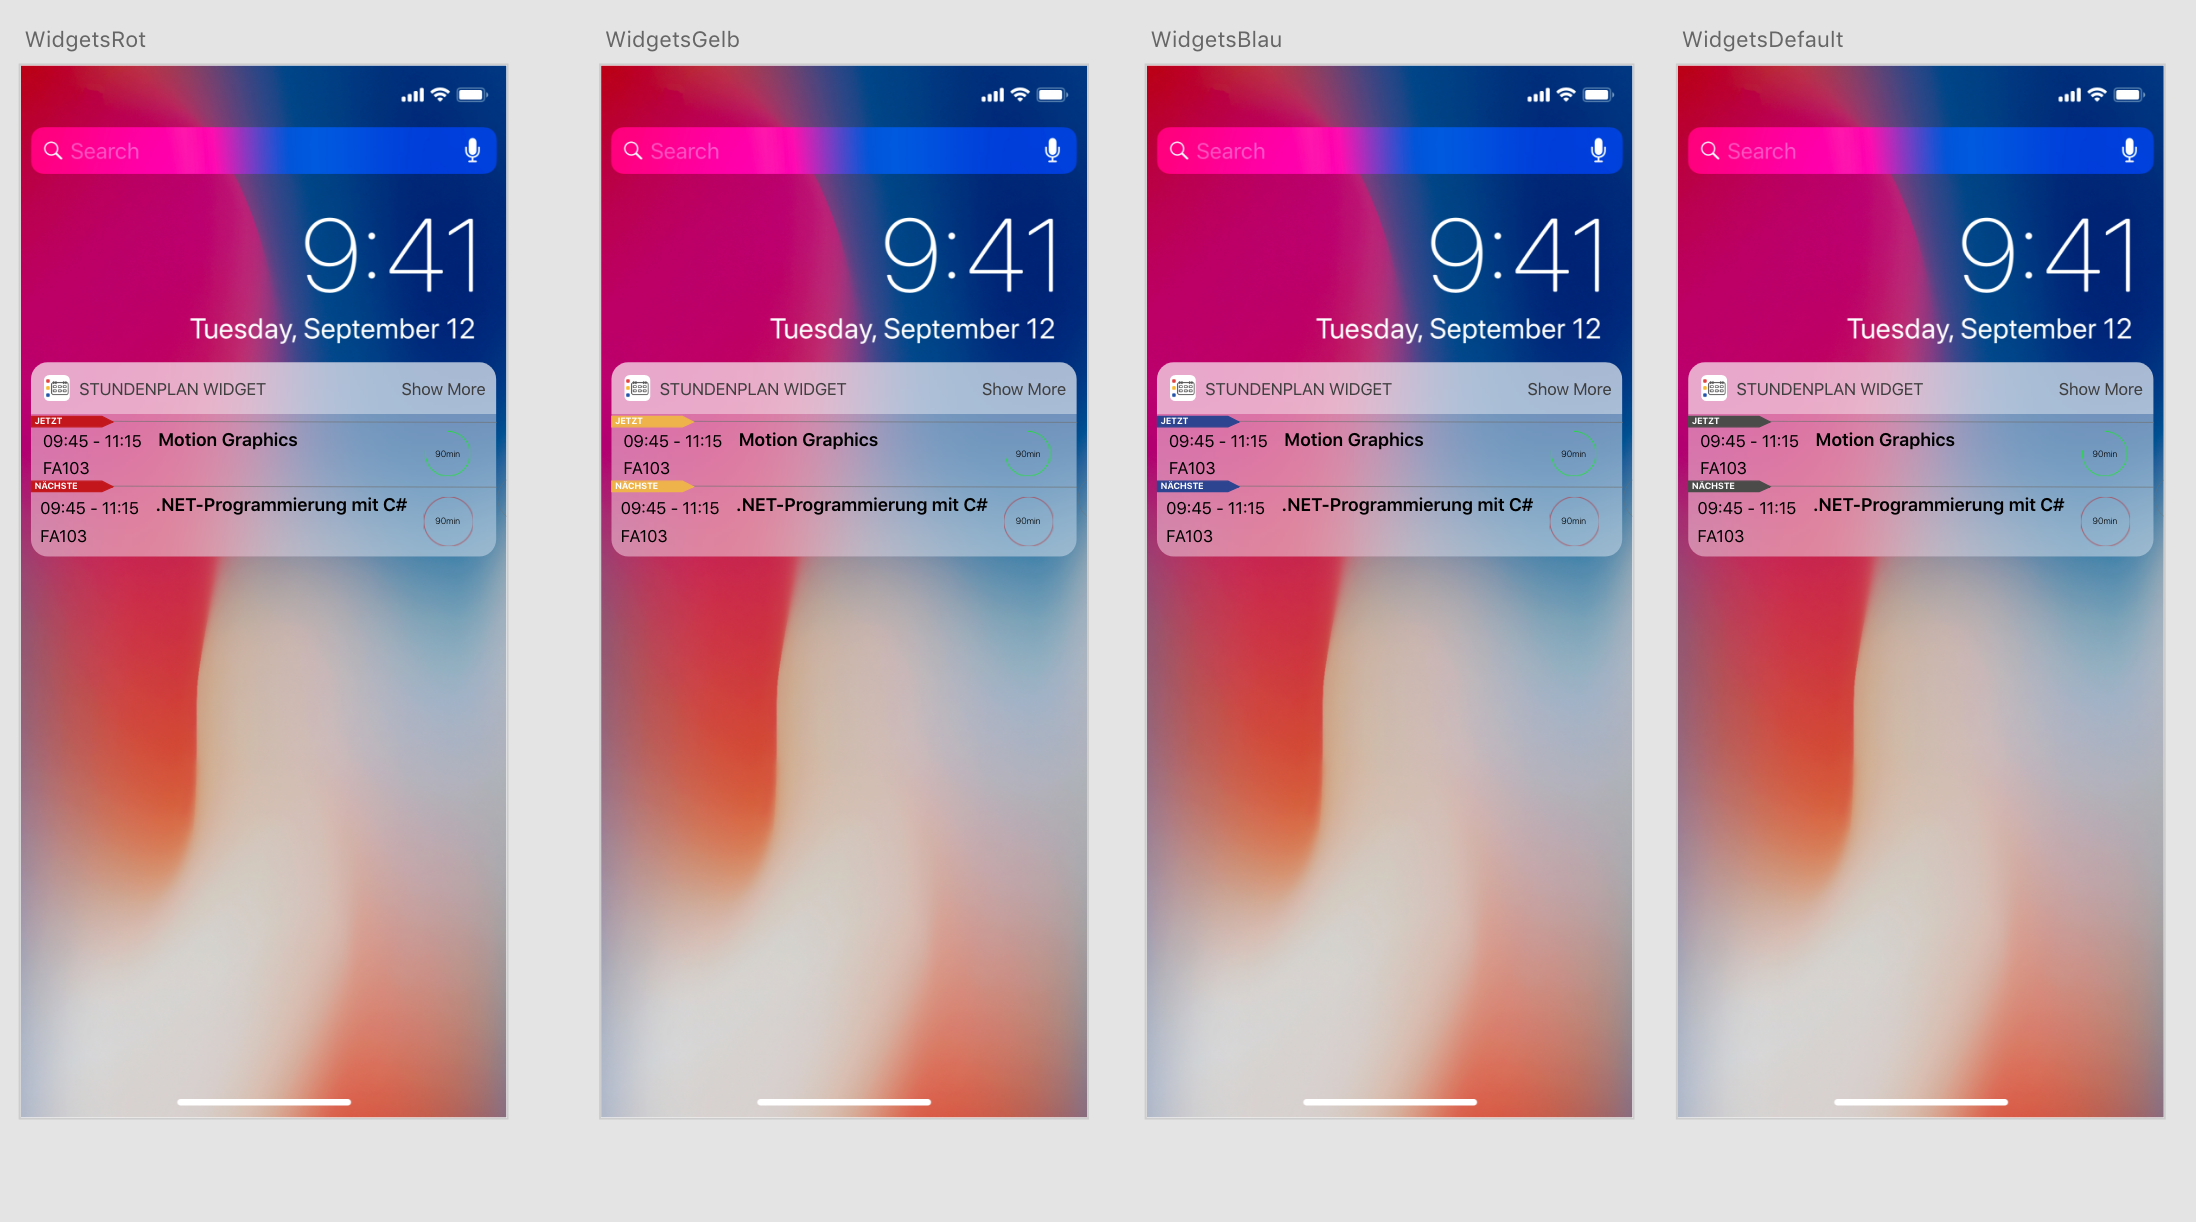
\includegraphics[scale=0.4]{WidgetDesign}}
	\caption{Design Widget 2}
	\label{fig1}
\end{figure}

Es wurde entschieden die Stundenplanapp durch ein Widget zu erweitern. Deshalb wurde auch ein Widget Designkonzept zur Ansicht der zwei folgenden Vorlesungen entwickelt. Ein sich füllender Kreis, mit verbleibender Zeitangabe, in der rechten Seite der Widgetzelle gibt Aufschluss über den zeitlichen Fortschritt der aktuellen Vorlesung.


\section{Entwicklung eines digitalen Prototypen}
Um die entwickelten Designentwürfe mit dem Entwicklerteams besser zu kommunizieren, wurde mithilfe des Design und Prototyping Programm Adobe XD ein digitaler Prototyp entwickelt. Mithilfe des digitalen Prototyp ist es möglich die angesetzten Designentwürfe in einem Click-Dummy auszuprobieren.

\begin{figure}[H]
	\centering
  \frame{ 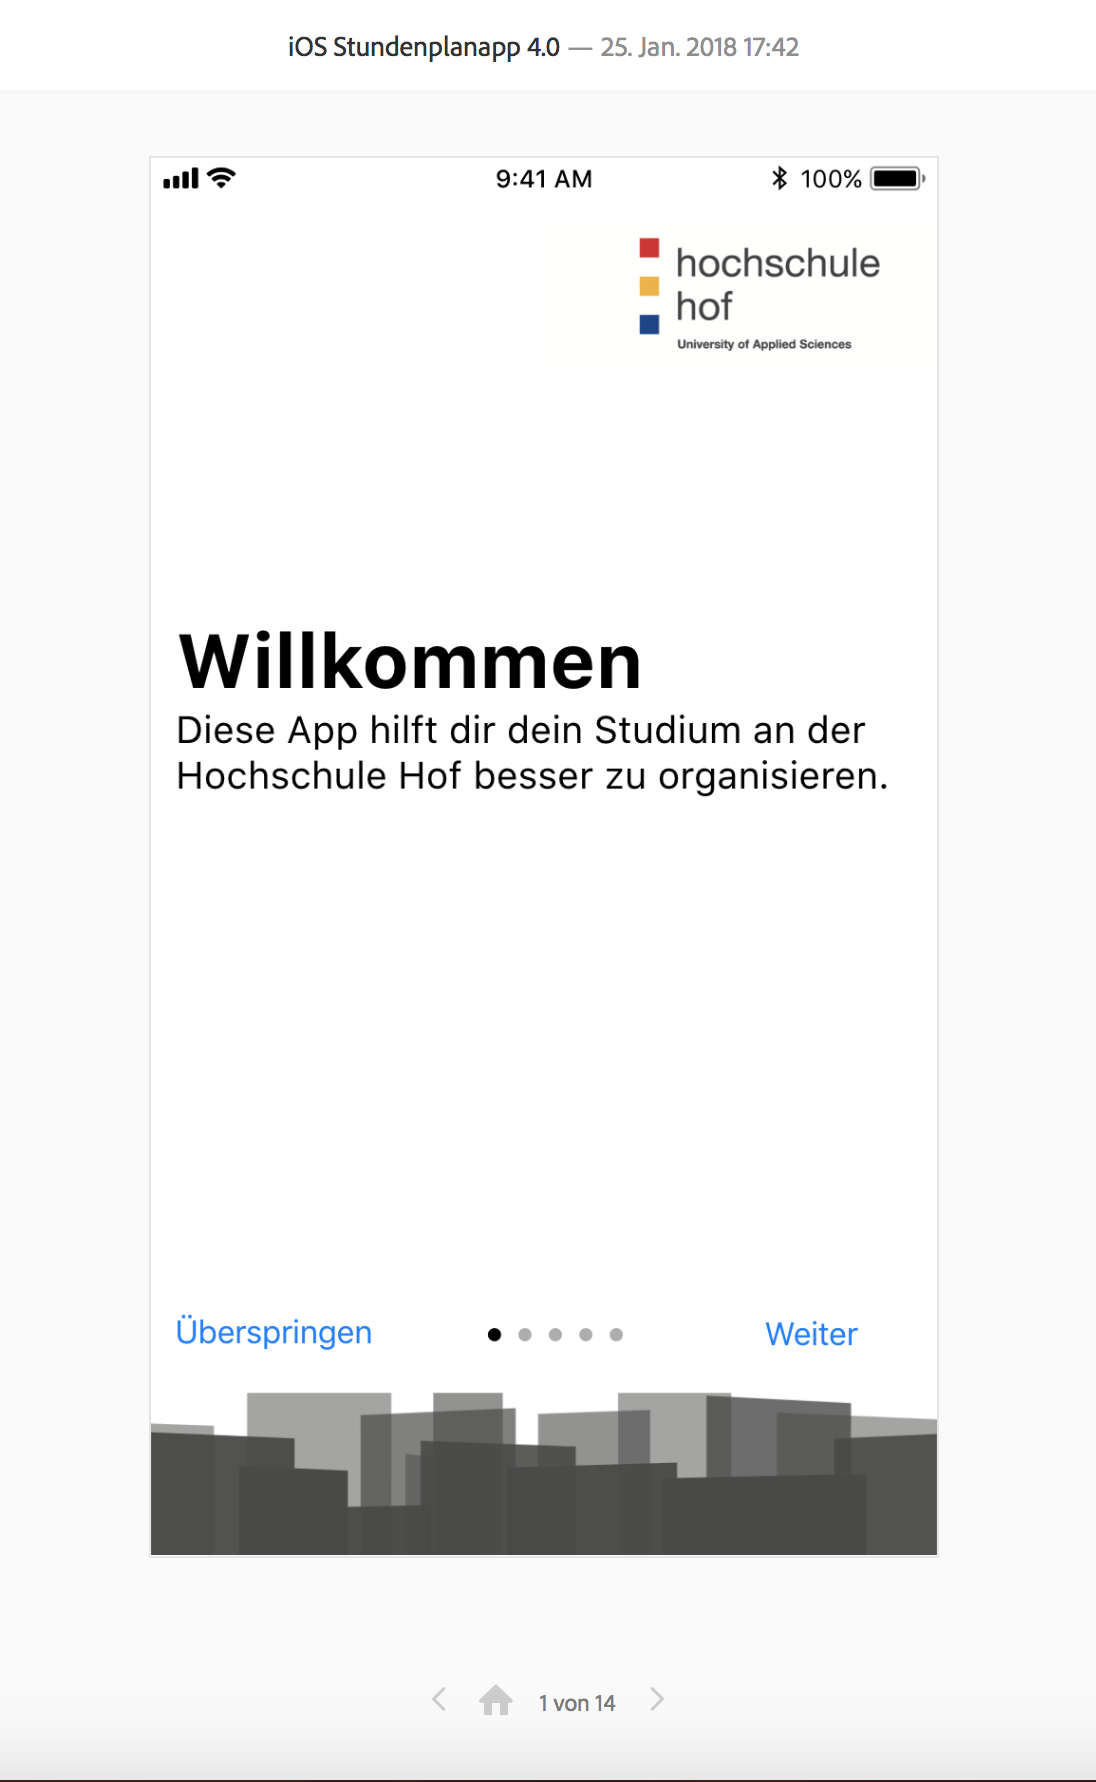
\includegraphics[scale=0.3]{design_digitalPrototype}}
	\caption{digitaler Prototyp}
	\label{fig1}
\end{figure}

Link zum digitalen Prototypen:\\
\url{https://xd.adobe.com/view/9cd14a5a-1e60-47c7-836d-6343e4d0784d}

